\documentclass{article}

%\usepackage{xcolor}
\usepackage[T1]{fontenc}
\usepackage{palatino}
\usepackage{courier}
\usepackage{alltt}
\usepackage{longtable}
%\DeclareTextSymbol{\QT}{T1}{39}
%\DeclareTextSymbol{\COMMA}{T1}{44}
%\DeclareTextSymbol{\COLON}{T1}{58}
%\DeclareTextSymbol{\SC}{T1}{59}
%\DeclareTextSymbol{\BS}{T1}{92}
%\DeclareTextSymbol{\CI}{T1}{94}
%\DeclareTextSymbol{\TI}{T1}{126}
%\definecolor{navy}{rgb}{0.15, 0.15, 0.45} 
%\definecolor{myblue}{rgb}{0.25, 0.25, 0.645} 
%\definecolor{darkred}{rgb}{0.845, 0.125, 0.125} 
%\definecolor{grey}{rgb}{0.4, 0.4, 0.4} 
%\definecolor{darkgreen}{rgb}{0.125, 0.845, 0.125} 
%\definecolor{leaf}{rgb}{0.1, 0.9, 0.1} 
%
%\newcommand{\mlkeywordA}[1]{\mbox{\color{cyan}{\textbf{\texttt{#1}}}}}
%\newcommand{\mlkeywordB}[1]{\mbox{\color{navy}{\textbf{\texttt{#1}}}}}
%\newcommand{\mlkeyword}[1]{\mbox{\color{red}{#1}}}
%\newcommand{\mloperator}[1]{\mbox{\color{darkgreen}{#1}}}
%\newcommand{\mlmodulename}[1]{\mbox{\color{navy}{#1}}}
%\newcommand{\mlstring}[1]{\mbox{\color{navy}{#1}}}
%\newcommand{\mlcomments}[1]{\mbox{\color{grey}{#1}}}
%\newcommand{\mlcodeline}[2]{\tiny\sl #1 & \begin{minipage}[c]{0.8\linewidth}\begin{alltt}\mbox{#2}\end{alltt}\end{minipage}\\}
% ---------------------------------------------------------------------

\usepackage{graphicx,enumerate,calc,ifthen}
\usepackage[french]{babel}
\usepackage[utf8]{inputenc}
\usepackage{float}
\floatstyle{boxed} 
\restylefloat{figure}

%%%%%%%%%%%%
% Document %
%%%%%%%%%%%%
\begin{document}

\title{Analyse des Besoins}
\author{Ghislain Loaec}
\maketitle

\begin{abstract}
Ce document vise à déterminer les objectifs de ce projet
\end{abstract}

\tableofcontents
\listoffigures
\listoftables
%\listofalgorithms

\section{Cahier des charges}
%%%%%%%%%%%%%%%%%%%%%%%%%%%%

\subsection{Objectifs}
\subsection{Contraintes}

\section{Analyse Conceptuelle}
%%%%%%%%%%%%%%%%%%%%%%%%%%%%%%

\subsection{Diagramme UML des cas d'utilisation}



\subsection{Diagramme UML des classes}

\begin{figure}[H]
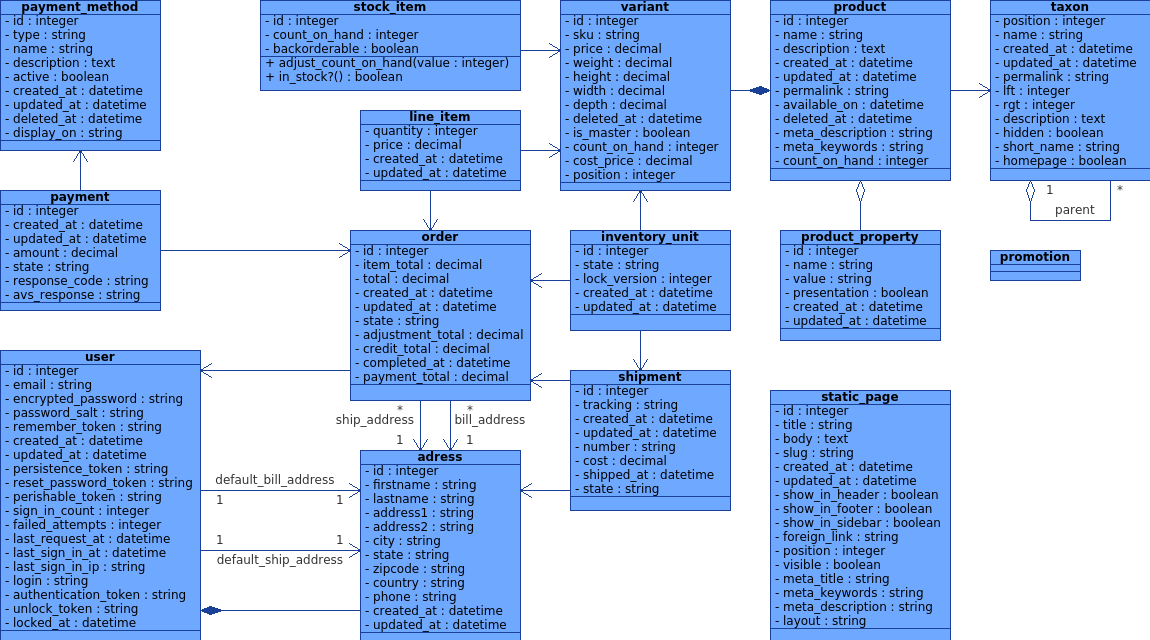
\includegraphics[width=\textwidth]{class_diagram.png} 
\caption{Diagramme des classes}
\label{class_diagram}
\end{figure}

\section{Choix Technologiques}
%%%%%%%%%%%%%%%%%%%%%%%%%%%%%%

\subsection{Languages de programmation}
\subsection{Approche MVC}


\section{Fonctionalités}
%%%%%%%%%%%%%%%%%%%%%%%%

\section{Tests Unitaires}
%%%%%%%%%%%%%%%%%%%%%%%%%


\end{document}
